\documentclass{article}
\usepackage[T2A]{fontenc}
\usepackage[utf8]{inputenc}
\usepackage[english,russian]{babel}
\usepackage{amsmath}
\usepackage{amssymb}
\usepackage{amsfonts}
\usepackage{xcolor}
\usepackage{enumitem}
\usepackage[top=2cm, bottom=4.5cm, left=2.5cm, right=2.7cm]{geometry}
\usepackage{lastpage}
\usepackage{fancyhdr}
%\usepackage{mathrsfs}
\usepackage{hyperref}
\usepackage[amsmath,thmmarks]{ntheorem}
\usepackage{cleveref}
%\usepackage{extarrows}
\usepackage{graphicx}
\usepackage{wrapfig}
\usepackage{subcaption}
\usepackage[section]{placeins}
%\usepackage{amsthm}

\newcommand{\rank}{\operatorname{rank}}

\newcommand{\prob}[1]{\item \textbf{(#1 баллов)}.}
\newcommand{\bonus}{\item \textbf{(Бонус)}.~}

\setlength{\parindent}{0.0in}
\setlength{\parskip}{0.05in}

\pagestyle{fancyplain}
\headheight 35pt           
\rhead{}
\chead{\textbf{\Large Домашняя работа 1} \\ (теория) \\  }
\lhead{ФКН ВШЭ \\ Основы Матричных Вычислений \\ Весенний семестр 2025} 
\lfoot{}
\cfoot{}
\rfoot{\small\thepage}
\headsep 1.5em

%\usepackage[thmmarks]{ntheorem}
\theoremheaderfont{\bfseries}
\theorembodyfont{\normalfont}
\theoremseparator{}
\theoremsymbol{$\blacksquare$}
\newtheorem*{proof}{$\square$}

\newcommand{\conj}[1]{\overline{#1}}
\newcommand{\R}{\mathbb{R}}
\renewcommand{\C}{\mathbb{C}}

\renewcommand{\leq}{\leqslant}
\renewcommand{\geq}{\geqslant}

\hypersetup{%
	pdfborder = {0 0 0}
}


\begin{document}
	\begin{center}
		Работу выполнил:
		
		\textbf{Назмиев Айрат, группа 1}
	\end{center}
	
	\section*{Задача 1}
	
	Пусть задан вектор $u\in\mathbb{C}^n\colon \|u\|_2=1$. Найдите все $\alpha \in \mathbb{C}$, для которых $A = I - \alpha u u^*$ является: 1) эрмитовой 2) косоэрмитовой 3) унитарной 4) нормальной. Для пункта~{3)} также нарисуйте найденные $\alpha$ на комплексной плоскости.
	
	\begin{proof} Найдем все $\alpha \in \mathbb{C}$ в каждом пункте. Обозначим $\alpha = a + ib,\;a,b\in\R$.
		\begin{enumerate}
			\item 
			$A$ --- эрмитова: $A^* = A$.
			
			$A^* = I - \conj\alpha u u^* = I - \alpha u u^* = A$, из условия $\|u\|_2=1$, значит $u u^*\neq 0$.
			
			$\alpha = \conj{\alpha} \iff \alpha \in \mathbb{R}$.
			
			\item
			$A$ --- косоэрмитова: $A^* = -A$.
			
			$A^* = I - \conj{\alpha} u u^* = -I + \alpha u u^* = -A$.
			
			$2I = (\alpha + \conj\alpha) u u^*$.
			
			$I$ имеет ранг $n$, тогда как $\rank{u u^*} = 1$ ($u \neq 0$), в этом случае $u u^* = u^* u = 1$. Значит, равенство может выполнятся только при $n=1$, в скалярном случае. Тогда также должно быть выполнено $2 = \alpha + \conj\alpha = 2a$. Получаем, что для $n\geq 1$ таких $\alpha$ не существует ($A$ не может быть косоэрмитовой), для $n=1$: $\alpha = 1 + ib,\;\forall b\in \R$.
			
			
			\item 
			$A$ --- унитарная: $A A^* = I$.
			
			$A A^* = (I -\alpha u u^*)(I -\conj\alpha u u^*) = I - (\alpha + \conj\alpha) u u^* + |\alpha|^2 u u^* u u^* = [u^* u = \|u\|_2 = 1] = I - (\alpha + \conj\alpha) u u^* + |\alpha|^2 u u^* = I$.
			
			$|\alpha|^2 u u^* = (\alpha + \conj\alpha) u u^*$.
			
			$a^2 + b^2 = 2a,\; (a-1)^2 + b^2 = 1$.
			
			Таким образом, $\alpha \in \{z\in\C:\:|z-1|=1\}$. Изобразим множество на комплексной плоскости: окружность радиуса 1 с центром в $z=1$.
			
			\begin{figure}[h!]
				\centering
				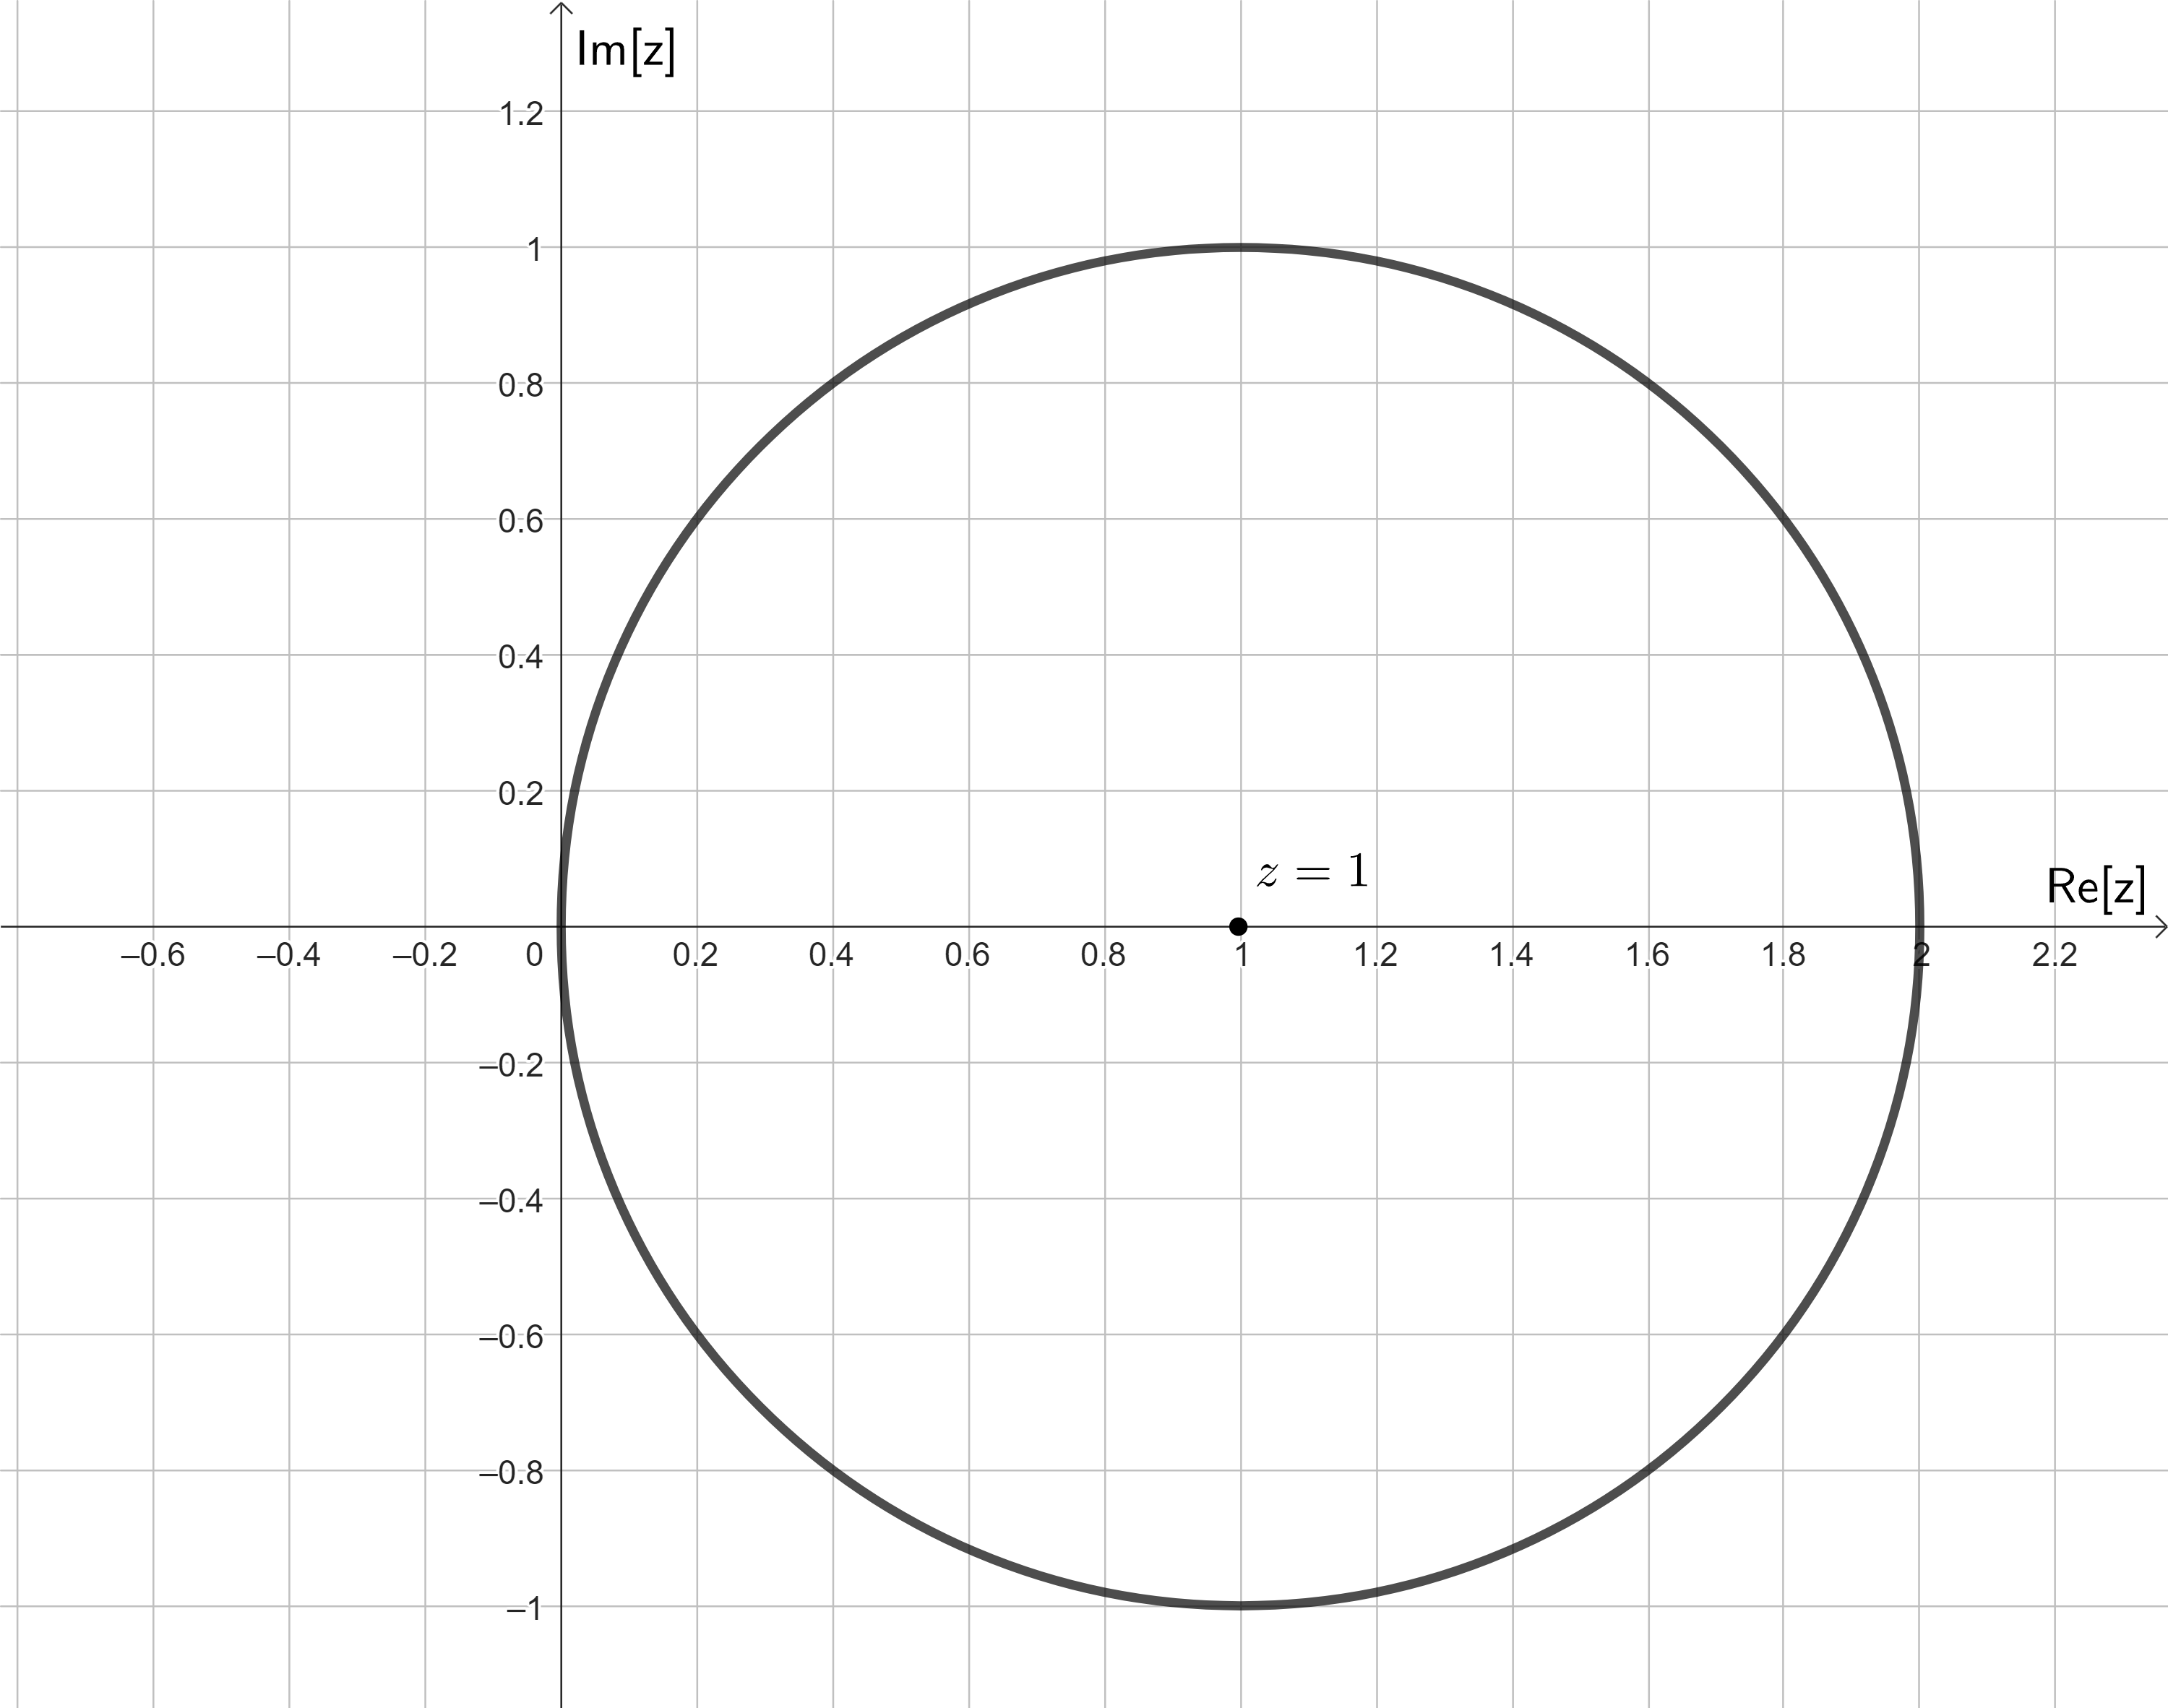
\includegraphics[width=0.3\linewidth]{figures/z-1}
			\end{figure}
			
			\item 
			$A$ --- нормальная, $AA^* = A^*A$.
			
			$AA^* = I - (\alpha + \conj\alpha) u u^* + |\alpha|^2 u u^*$; $A^* A = I - (\alpha + \conj\alpha) u u^* + |\alpha|^2 u u^*$.
			
			Можно видеть, что $AA^* = A^*A,\; \forall \alpha\in\C$.
		\end{enumerate}
	\end{proof}
	
	\section*{Задача 2}
	\begin{enumerate}
		\item
		Докажите, что для любой косоэрмитовой $K\in\mathbb{C}^{n\times n}$ матрица:
		\begin{equation} \label{eq:caley}
			Q = (I - K)^{-1} (I+K)
		\end{equation}
		будет унитарной. 
		\item Найдите множество всех унитарных матриц, которые представимы в виде \eqref{eq:caley}.
	\end{enumerate}
	
	\begin{proof}
		Для начала покажем, что матрица $I - K$ является обратимой. Известно, что собственные значения косоэрмитовых матриц имеет вид $\lambda(K) \in i\R$, то есть являются чисто мнимыми, в том числе могут равняться нулю. Пусть $K = U \Lambda U^{-1} = U \Lambda U^*$ --- ее собственное разложение в ОНБ комплексного векторного пространства (косоэрмитовы матрицы нормальные). Тогда матрицу можно расписать в следующем виде: $I - K = U U^* - U \Lambda U^* = U (I - \Lambda) U^*$, то есть $I - K$ имеет собственные значения вида $\lambda(I - K) = 1 - \lambda(K) \neq 0$. Таким образом, все собственные значения данной матрицы ненулевые, а значит, $I - K$ обратима.
		
		
		Покажем, что матрица вида \eqref{eq:caley} является унитарной, для этого требуется доказать $Q Q^* = I$. Для этого воспользуемся известными свойствами: $(AB)^*=B^*A^*,\; (A^{-1})^* = (A^*)^{-1}$, свойством $K^* = -K$. Получим:
		\begin{equation*}\begin{aligned}
				Q^* &= (I - K)(I + K)^{-1},\\
				Q Q^* &= (I - K)^{-1}(I + K)(I - K)(I + K)^{-1}.
		\end{aligned}\end{equation*}
		Докажем простой факт: матрицы вида $I - A$ и $I + A$ коммутируют $\forall A \in \C$. Действительно:
		\begin{equation*}\begin{aligned}
				(I + A)(I - A) = I - A^2 = (I - A)(I + A).
		\end{aligned}\end{equation*}
		Поэтому можно переставить в $Q Q^*$ второй и третий множитель местами:
		\begin{equation*}\begin{aligned}
				Q Q^* = (I - K)^{-1}(I - K)(I + K)(I + K)^{-1} = I, 
		\end{aligned}\end{equation*}
		что и требовалось.
		
		Было доказано, что для любой косоэрмитовой $K \in \C^{n\times n} $ формула \eqref{eq:caley} задает унитарную $Q$.
		
		Теперь найдем множество унитарных матриц, представимых в виде \eqref{eq:caley}.
		
		Известно, что в общем случае собственные числа косоэрмитовых матриц чисто мнимые, а ортогональных --- являются комплексными и равны единице по модулю.
		
		Пусть $v$ --- собственный вектор $K$: $Kv = \lambda v$, $\lambda \in i\R$. Тогда:
		\begin{equation}\begin{aligned}\label{eq:Qv_prefinal}
				Qv = (I - K)^{-1}(1 + \lambda) v.
		\end{aligned}\end{equation}
		Известно, что собственные векторы матрицы и обратной матрицы совпадают, при этом соответствующим данному вектору собственным значением обратной матрицы будет обратное собственное число исходной матрицы:
		\begin{equation*}\begin{aligned}
				Ax = \lambda x,\; x = \lambda A^{-1} x,\; \lambda^{-1} x = A^{-1} x.
		\end{aligned}\end{equation*}
		Значит, если $v$ - собственный для $K$, то он собственный как для $(I - K)$:
		\begin{equation*}\begin{aligned}
				(I - K) v = (1 - \lambda)v, 
		\end{aligned}\end{equation*}
		так и для $(I - K)^{-1}$:
		\begin{equation*}\begin{aligned}
				(I - K)^{-1} v = \dfrac{1}{1-\lambda} v.
		\end{aligned}\end{equation*}
		Таким образом, \eqref{eq:Qv_prefinal} можно записать в виде:
		\begin{equation}
			Qv = \frac{1 + \lambda}{1 - \lambda} v = \mu v,
		\end{equation}
		что означает, $Q$ имеет те же собственные векторы $v$, что и $K$, которым соответствует собственное число $\mu = (1 + \lambda)(1 - \lambda)^{-1}$. 
		
		Введем обозначение $\lambda = i b,\; b\in\R$. Определим, какие значения может принимать $\mu$:
		
		\begin{equation} \label{eq:mu_b}
			\mu = \frac{1 + ib}{1 - ib} = \frac{(1-b^2) + 2ib}{1+b^2}.
		\end{equation}
		
		Можно легко убедится, что $|\mu|=1$, то есть собственные значения лежат на единичной окружности:
		
		\begin{equation*}
			|\mu| = \left|\frac{(1-b^2) + 2ib}{1+b^2}\right| = \sqrt{\frac{(1-b^2)^2 + (2b)^2}{(1+b^2)^2}} = \sqrt{\frac{1 -2b^2+b^4+4b^2}{(1+b^2)^2}} = 1.
		\end{equation*}
		
		Введем обозначение $\mu = e^{i\theta} = \cos(\theta) + i \sin(\theta)$. Из \eqref{eq:mu_b} получаем, что $\cos(\theta) = (1-b^2)(1+b^2)^{-1}$, $\sin(\theta) = 2b (1+b^2)^{-1}$. Зададимся вопросом, какие значения может принимать $\mu$ на единичной окружности.
		
		\begin{figure}[h!]
			\centering
			\begin{subfigure}[h]{0.45\linewidth}
				\centering
				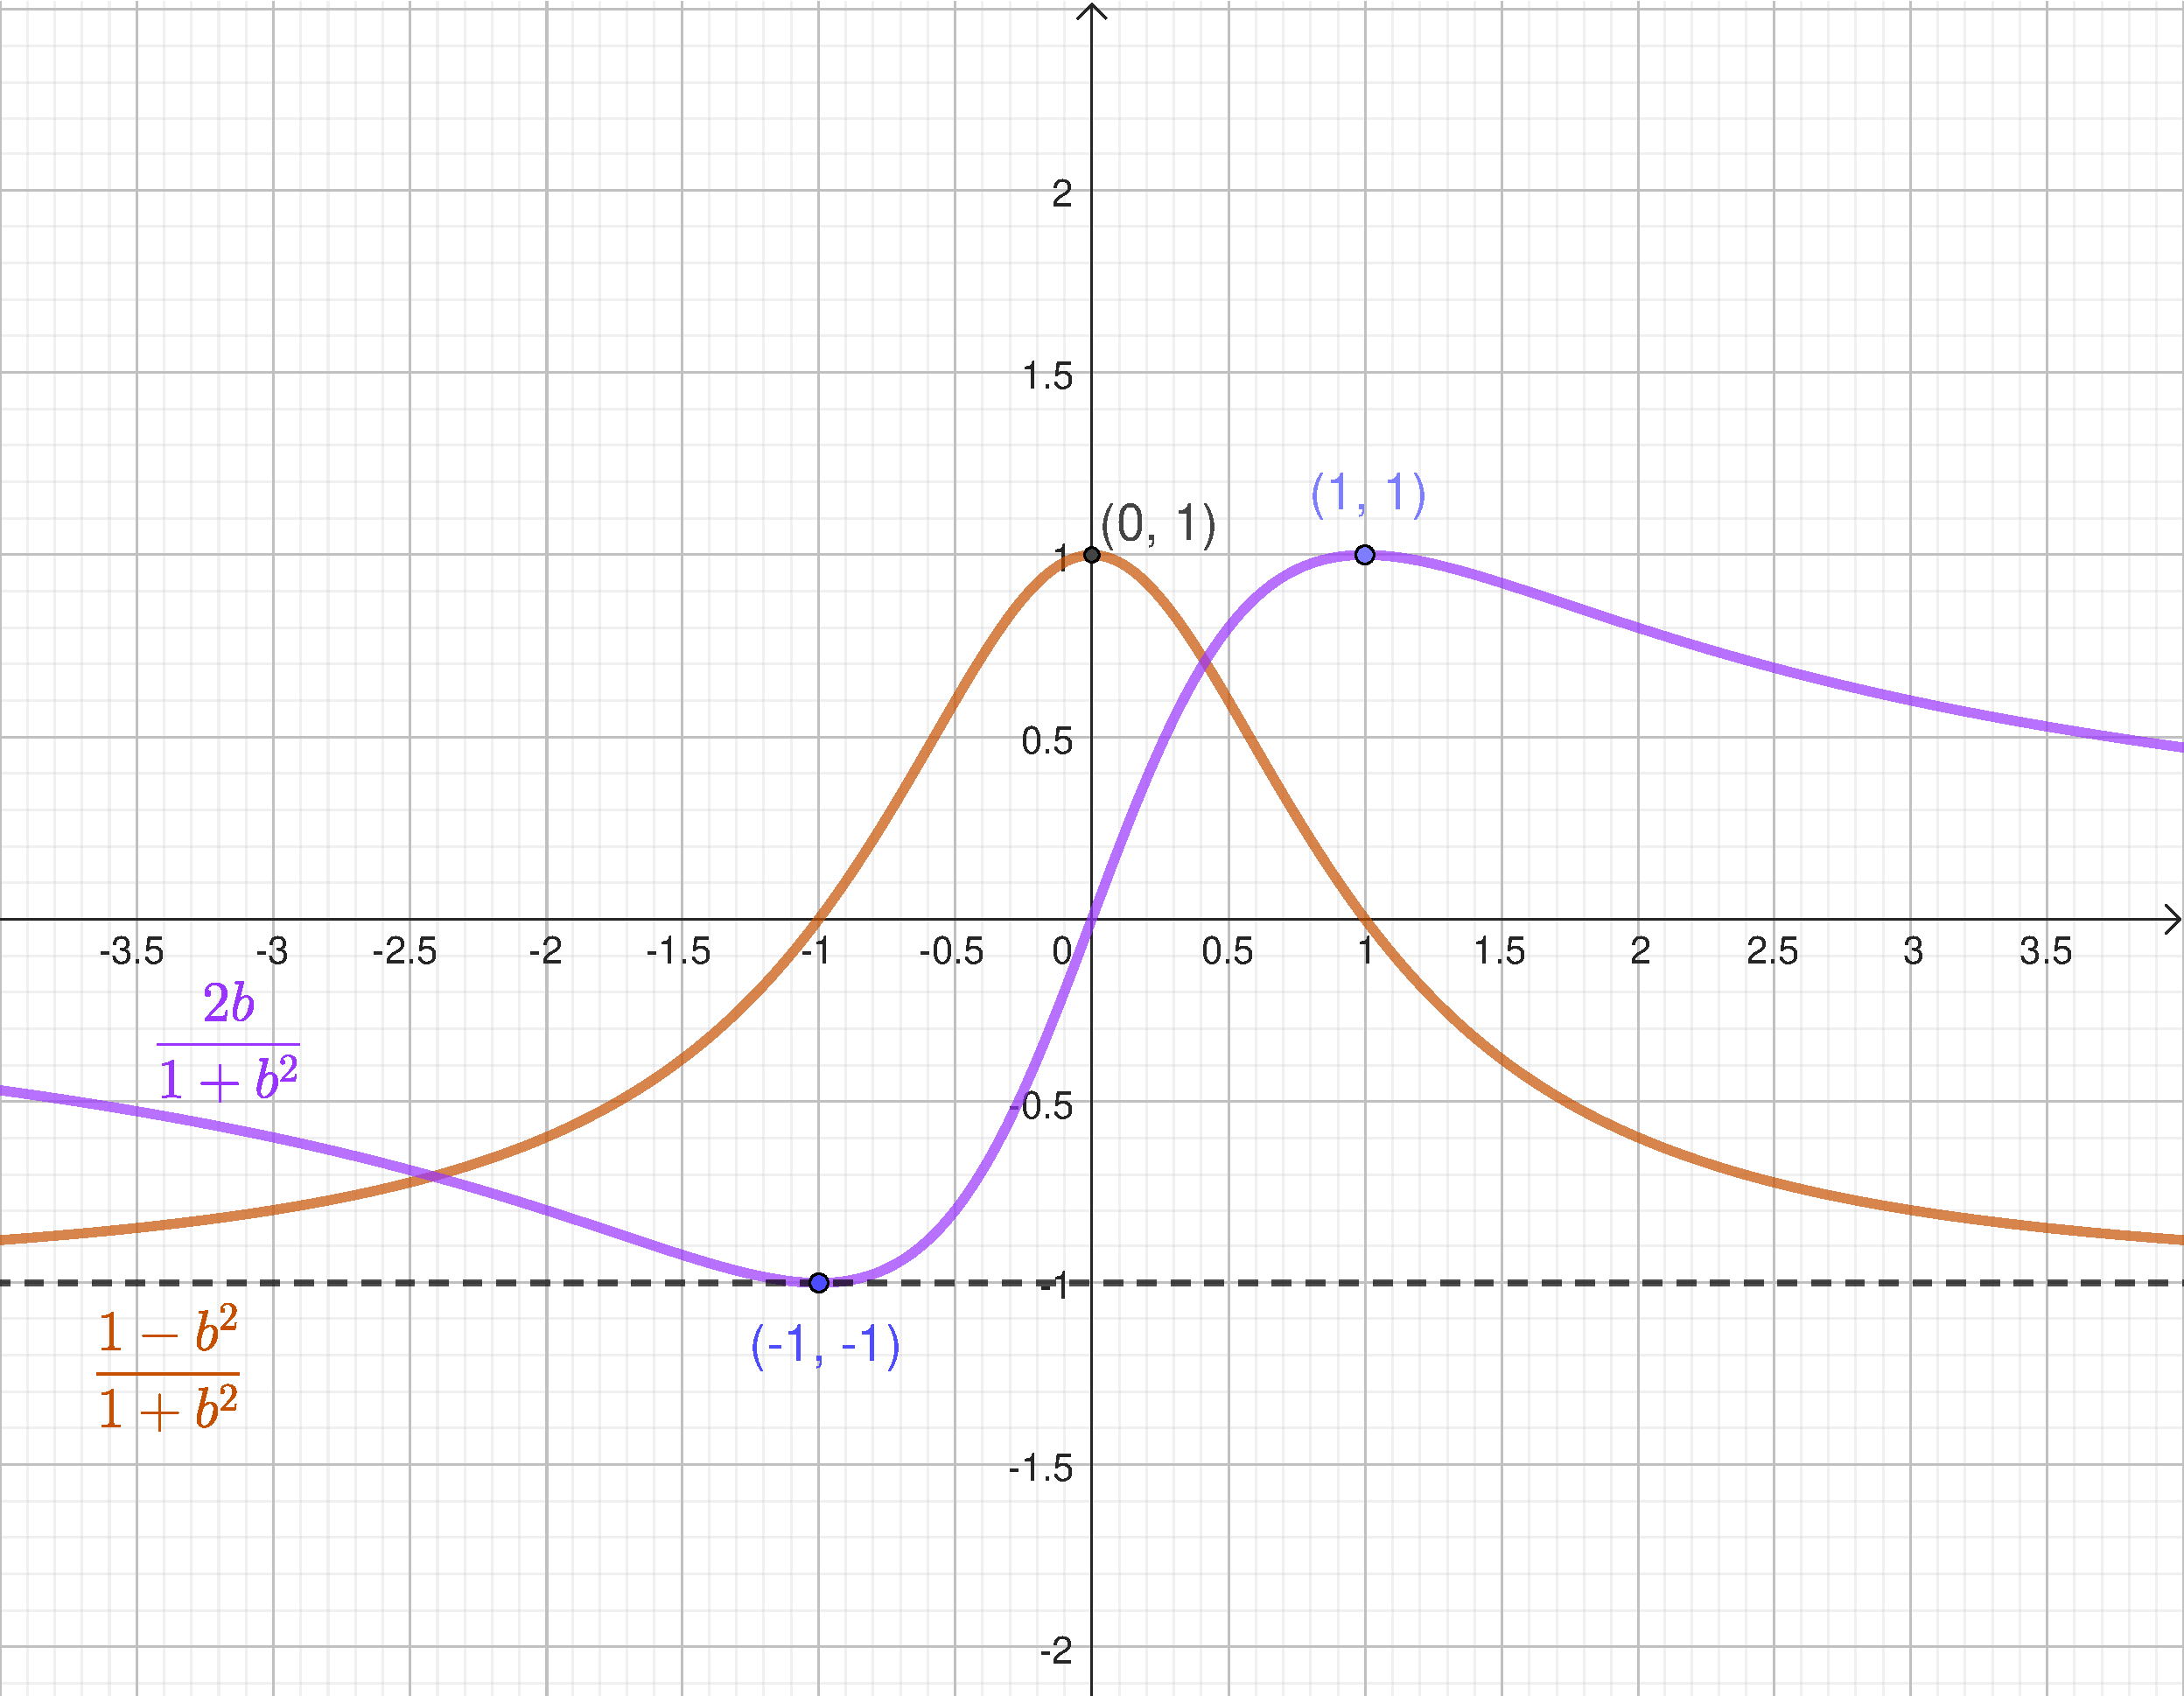
\includegraphics[width=\linewidth]{figures/mu_sin_cos}
				\subcaption{Графики $\frac{1-b^2}{1+b^2}$ и $\frac{2b}{1+b^2}$}
			\end{subfigure}
			\hfill
			\begin{subfigure}[h]{0.35\linewidth}
				\centering
				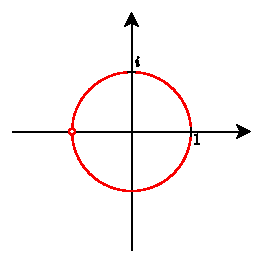
\includegraphics[width=\linewidth]{figures/muQ}
				\subcaption{$\mu$ на комплексной плоскости}
			\end{subfigure}
		\end{figure}
		
		Можно легко показать тот факт, что в параметризации \eqref{eq:mu_b} невозможно задать точку $\mu=-1$. Доказывается это средствами матанализа, исследуя нули, экстремумы, участки монотонности и асимптоты функций $x(b)=(1-b^2)(1+b^2)^{-1}$ и $y(b)=2b (1+b^2)^{-1}$, но выкладки оказываются крайне громоздкими, поэтому здесь не приводятся. Вместо этого приведены графики функций и полученное множество допустимых значений $\mu$ на $\C$. Можно видеть, что при изменении $b\in\R$ достигаются все точки на единичной окружности, $(x(b), y(b)),\; x^2(b)+y^2(b)=1$, кроме $(-1, 0)$: она не достигается и является пределом при $b\rightarrow \pm \infty$. То есть $\mu \in \{z\in\C:\: |z|=1,\; z\neq -1\}$.
		
		Вместо описанного выше наброска доказательства ГМТ $\mu$ можно заметить, что \eqref{eq:mu_b} является преобразованием Кэли в скалярном случае, которое отображает мнимую ось на комплексной плоскости в единичную окружность, при этом $\pm i \infty$ отображается в $-1$. Кстати, в задаче изначально рассматривается более общее отображение Кэли: для комплексных матриц, в приложении к параметризации унитарных матриц через косоэрмитовы. 
		
		Таким образом, вид \eqref{eq:caley} описывает множество всех унитарных матриц $Q\in\C^{n\times n}$, которые не имеют собственного значения $-1$.
	\end{proof}
	
	\section*{Задача 3}
	Докажите, что
	\[
	\|A\|_{1\to 2} \leq  \|A\|_{2} \leq \sqrt{n} \|A\|_{1\to 2
	}, \quad \forall A\in\mathbb{C}^{m\times n}.
	\] 
	\textbf{Указание:} В случае использования констант эквивалентности векторных норм необходимо обосновывать это значение констант. 
	
	\begin{proof}		
		Докажем, что $\|x\|_2 \leq \|x\|_1 \leq \sqrt{n}\|x\|_2$, для этого воспользуемся полуаддитивностью квадратного корня и неравенством КБШ:
		\begin{equation*}
			\|x\|_2 = \sqrt{\sum\limits_{i=1}^n |x_i|^2} \leq \sum\limits_{i=1}^n \sqrt{|x_i|^2} = \sum\limits_{i=1}^n |x_i| = \|x\|_1 = \sum\limits_{i=1}^n |x_i| \cdot 1 \leq \sqrt{\sum\limits_{i=1}^n |x_i|^2} \cdot \sqrt{\sum\limits_{i=1}^n 1^2} = \sqrt{n} \|x\|_2.
		\end{equation*}
		Выпишем определения операторных норм:
		\begin{equation*}
			\|A\|_{1\to2} = \sup\limits_{\|x\|_1=1} \|Ax\|_{2},\quad \|A\|_{2} = \sup\limits_{\|x\|_2=1} \|Ax\|_{2}
		\end{equation*}
		Далее докажем первое неравенство в условии задачи: $\|A\|_{1\to 2} \leq  \|A\|_{2}$. Из определения операторной нормы ($\forall x\in\C^n$, $\|x\|_1=1$ выполнено $\|x\|_2 \leq \|x\|_1=1$) и доказанных неравенств на векторные нормы следует, что:
		\begin{equation*}
			\|Ax\|_2 \leq \|A\|_2 \|x\|_2 \leq \|A\|_2 \|x\|_1 =  \|A\|_2 \cdot 1 \leq  \|A\|_2.
		\end{equation*}
		Взяв супремум по $\|x\|_1$ на единичной сфере, можно получить:
		\begin{equation*}
			\|A\|_{1\to2} = \sup\limits_{\|x\|_1=1} \|Ax\|_2  \leq \|A\|_2,
		\end{equation*}
		что и требовалось. Перейдем к доказательству второго неравенства, $\|A\|_{2} \leq \sqrt{n}\|A\|_{1\to 2}$. Вновь сошлемся на доказанные неравенства на векторные нормы ($\forall x\in\C^n$, $\|x\|_2=1$ выполнено $\|x\|_1 \leq \sqrt{n}\|x\|_2=\sqrt{n}$) и определения операторных норм и запишем:
		\begin{equation*}
			\|Ax\|_2 \leq \|A\|_{1\to2} \|x\|_1 \leq \|A\|_{1\to2} \sqrt{n} \|x\|_2 = \sqrt{n} \|A\|_{1\to2} 
		\end{equation*}
		Взяв супремум по $\|x\|_2$ на единичной сфере, можно получить:
		\begin{equation*}
			\|A\|_{2} = \sup\limits_{\|x\|_2=1} \|Ax\|_2  \leq \sqrt{n}\|A\|_{1\to2},
		\end{equation*}
		оба неравенства доказаны.
	\end{proof}
	\section*{Задача 4}
	Обозначим $A = \begin{bmatrix}0 & 1 \\ 0 & 0 \end{bmatrix}$ и $A_n = \begin{bmatrix} 0 & 1 \\ 1/n & 0 \end{bmatrix}, n\in\mathbb{N}$.
	\begin{enumerate}
		\item Обоснуйте сходимость $A_n\to A$, $n\to\infty$ исходя из определения сходимости с помощью норм.
		\item Найдите собственные разложения $A_n = S_n \Lambda_n S_n^{-1}$ и проверьте существование пределов для каждой из $S_n$,$\Lambda_n$ и $S_n^{-1}$. Почему не у всех из этих матриц существует предел?
		\item Найдите разложения Шура $A_n = U_n T_n U_n^{-1}$ и проверьте существование пределов для каждой из $U_n$,$T_n$ и $U_n^{-1}$.
	\end{enumerate}
	\begin{proof}
		Докажем сходимость $A_n\to A$, $n\to\infty$. Так как все матричные нормы в конечномерных пространствах эквивалентны, поэтому для удобства будем показывать сходимости по норме Фробениуса:
		\begin{equation*}
			\|A - A_n\|_F = \frac{1}{n} \rightarrow 0,\; n\rightarrow\infty,
		\end{equation*}
		то есть $A_n$ сходится к $A$.
		
		Найдем собственные разложение $A$ и $A_n$.
		\begin{equation*}\begin{aligned}
				\det(A-\lambda I) = \lambda^2=0,\quad \lambda_1=\lambda_2=0,\quad (A-0\cdot I) v = 0,\quad
				\begin{bmatrix}
					0 & 1\\ 0 & 0
				\end{bmatrix} v = 0,\quad v=\begin{bmatrix}
					1\\ 0
				\end{bmatrix},
		\end{aligned}\end{equation*}
		можно видеть, что у матрицы $A$ только один линейно независимый собственный вектор (а не 2), то есть у $A$ не имеет собственного разложения. При этом ЖНФ $A$ имеет вид:
		\begin{equation*}\begin{aligned}
				A = P J P^{-1},\quad J = \begin{bmatrix}
					0 & 1\\ 0 & 0
				\end{bmatrix},\quad P = P^{-1} = I
		\end{aligned}\end{equation*}
		Собственное разложение $A_n$: 
		\begin{equation*}\begin{aligned}
				&\det(A_n-\lambda I) = \lambda^2-\frac{1}{n}=0,\quad \lambda_{n1}=\frac{1}{\sqrt{n}},\quad \lambda_{n2}=-\frac{1}{\sqrt{n}},\quad (A-0\cdot I) v = 0,\quad
				v_{n1}=\begin{bmatrix}
					\sqrt{n}\\ 1
				\end{bmatrix},\quad v_{n2}=\begin{bmatrix}
					-\sqrt{n}\\ 1
				\end{bmatrix};\\
				& \Lambda_n = \begin{bmatrix}
					\frac{1}{\sqrt{n}} & 0 \\ 0 & -\frac{1}{\sqrt{n}}
				\end{bmatrix},\quad
				S_n = \begin{bmatrix}
					\sqrt{n} & -\sqrt{n}\\1 & 1
				\end{bmatrix},\quad 
				S_n^{-1} = \begin{bmatrix}
					\frac{1}{2\sqrt{n}} & \frac{1}{2}\\ -\frac{1}{2\sqrt{n}} & \frac{1}{2}
				\end{bmatrix}
		\end{aligned}\end{equation*}
		Можно легко видеть (например, рассмотрев разницу матриц в норме Фробениуса), что последовательности $\Lambda_n$ и $S_n^{-1}$ имеют предел, а $S_n$ --- нет (так как некоторые элементы матрицы стремятся к бесконечности):
		\begin{equation*}\begin{aligned}
				\Lambda_n\xrightarrow[n\to\infty]{} 0,\quad
				S_n^{-1} \xrightarrow[n\to\infty]{}
				\begin{bmatrix}
					0 & \frac{1}{2}\\ 0 & \frac{1}{2}
				\end{bmatrix}.
		\end{aligned}\end{equation*}
		При этом $A_n = S_n \Lambda_n S_n^{-1}$ для любого \textit{конечного} $n$. Расходимость некоторых матриц (для выбранных собственных векторов --- расходимость $S_n$) связана с тем, что предел последовательности $A_n$ является вырожденной матрицей $A$, для которой не существует собственного разложения. При этом важно заметить, что сходимость собственных значений имеет место, $\lambda_{n1}$ и $\lambda_{n2}$ сходятся к 0.
		
		Теперь найдем разложения Шура матриц $A$ и $A_n$. 
		
		Для $A$ легко проверить, что можно записать разложение Шура, совпадающее с найденной выше ЖНФ:
		\begin{equation*}\begin{aligned}
				A = U T U^*,\quad T = \begin{bmatrix}
					0 & 1\\ 0 & 0
				\end{bmatrix},\quad U = U^* = I.
		\end{aligned}\end{equation*}
		Найдем разложение Шура для $A_n$. Нормируем найденный собственный вектор $v_1$, найдем для него ортогональный вектор и также его нормируем (вектора сформируют унитарную матрицу), далее найдем верхнетруегольную матрицу $T_n$:
		\begin{equation*}\begin{aligned}
				&v_{n1} = \begin{bmatrix}
					\sqrt{n}\\ 1
				\end{bmatrix},\quad
				v_{n2} = \begin{bmatrix}
					-1\\ \sqrt{n}
				\end{bmatrix},\quad
				u_{ni} = \frac{v_{ni}}{\|v_{ni}\|_2},\; i=1,2,\\
				&U_n = \begin{bmatrix}
					\frac{\sqrt{n}}{\sqrt{n+1}} & -\frac{1}{\sqrt{n+1}}\\ \frac{1}{\sqrt{n+1}} & \frac{\sqrt{n}}{\sqrt{n+1}}
				\end{bmatrix},\quad U_n^{-1} = U_n^*,\quad
				T_n = U_n^* A_n U_n = \begin{bmatrix}
					\frac{1}{\sqrt{n}} & \frac{n-1}{n}\\ 0 & -\frac{1}{\sqrt{n}}
				\end{bmatrix}\\
				&U_n, U_n^*\xrightarrow[n\to\infty]{} I = U, \quad T_n\xrightarrow[n\to\infty]{} \begin{bmatrix}
					0 & 1\\ 0 & 0
				\end{bmatrix} = T.
		\end{aligned}\end{equation*}
		Легко видеть, что полученные матрицы имеют пределы (например, это можно показать через фробениусовскую норму), при этом они совпадают с разложением Шура матрицы $A$, к которой стремится $A_n$. Таким образом можно заключить, что все матрицы в разложении Шура $A_n$ сходятся к соответствующим матрицам в разложении предельной матрицы $A$. 
	\end{proof}
	
	\textbf{Начиная со следующей задачи решения задач будут приведены в письменном виде.}
	
	\begin{figure}[h!]
		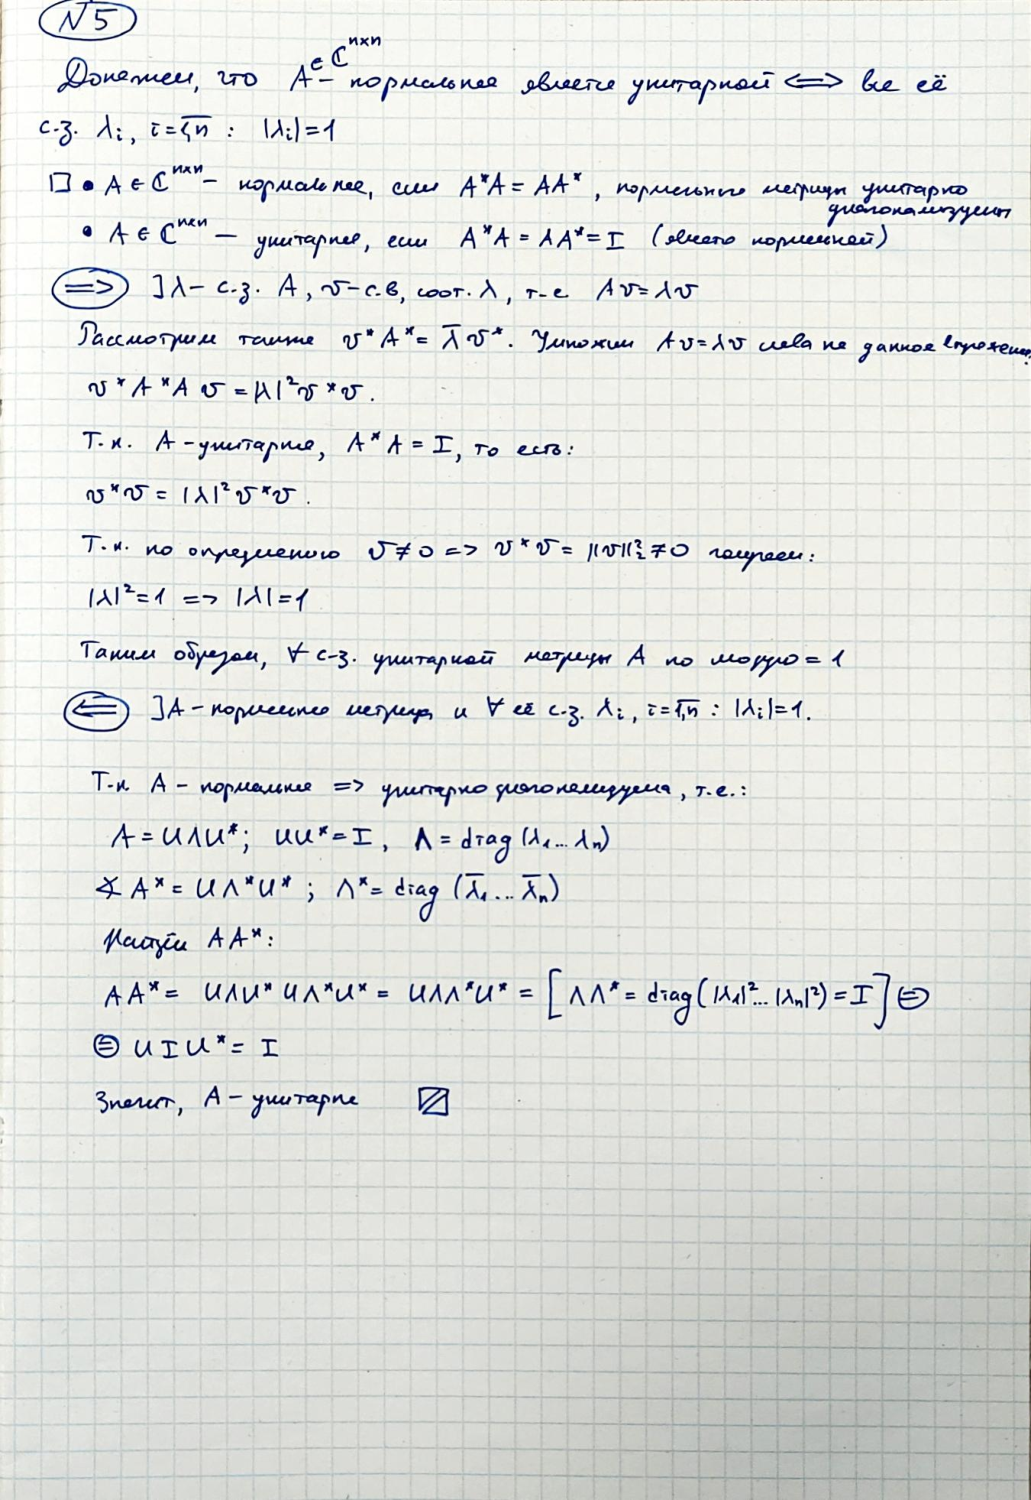
\includegraphics[width=0.95\linewidth]{handwritten/matcomp_hw1_5}
	\end{figure}
	
	\begin{figure}[h!]
		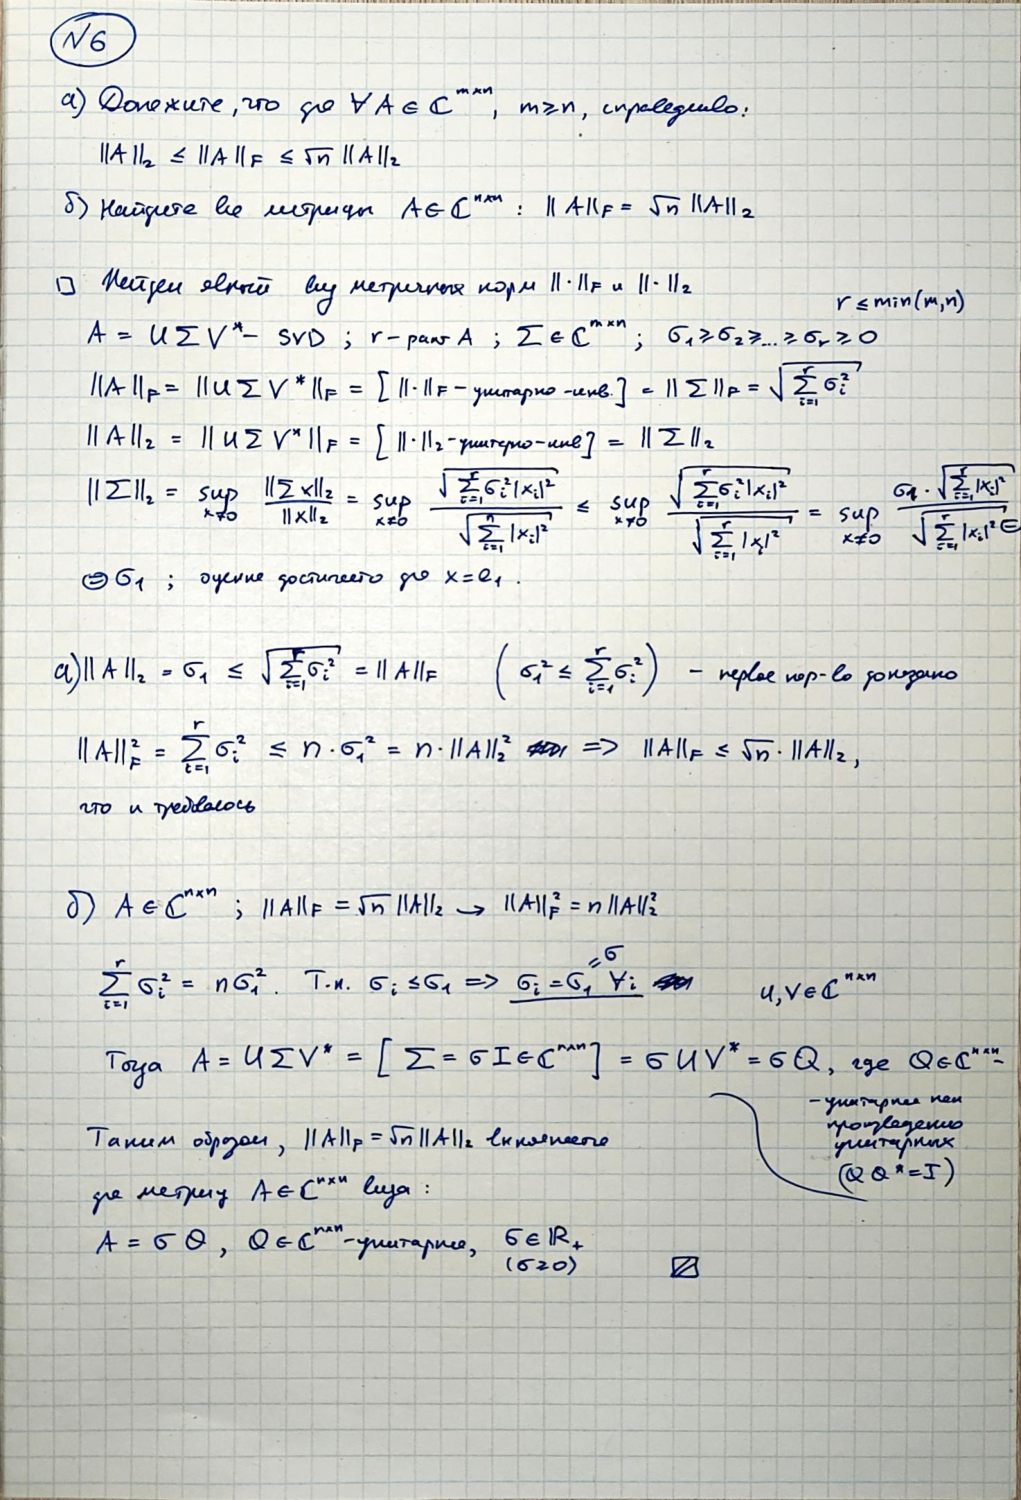
\includegraphics[width=0.95\linewidth]{handwritten/matcomp_hw1_6}
	\end{figure}
	
	\begin{figure}[h!]
		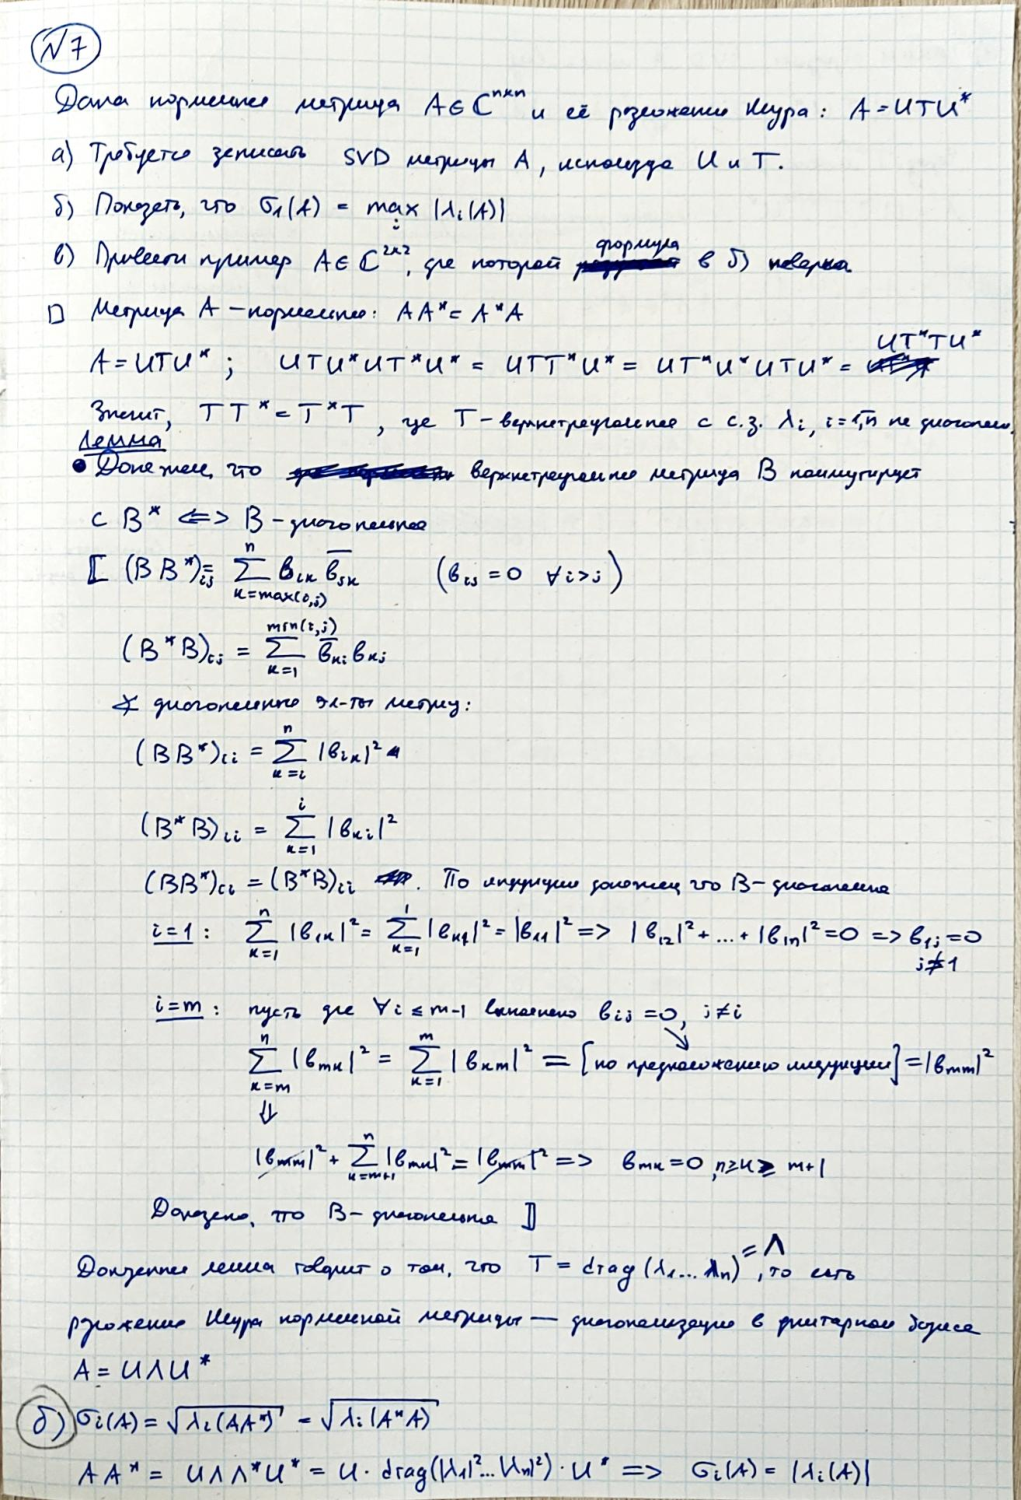
\includegraphics[width=0.95\linewidth]{handwritten/matcomp_hw1_7a}
	\end{figure}
	
	\begin{figure}[h!]
		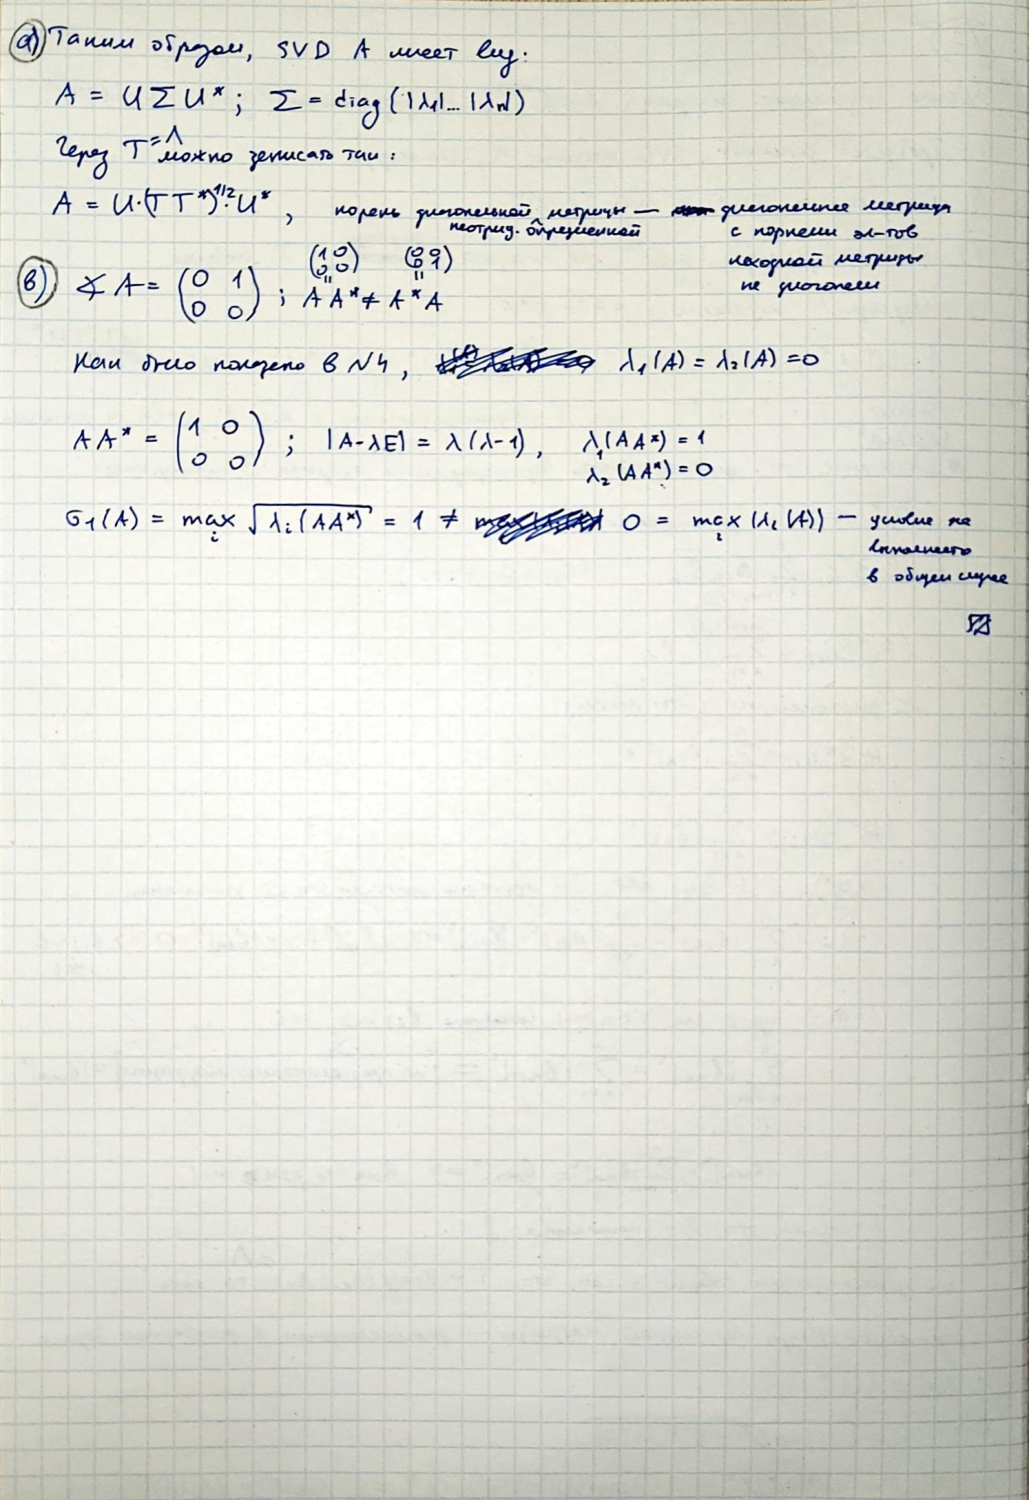
\includegraphics[width=0.95\linewidth]{handwritten/matcomp_hw1_7b}
	\end{figure}
	
	\begin{figure}[h!]
		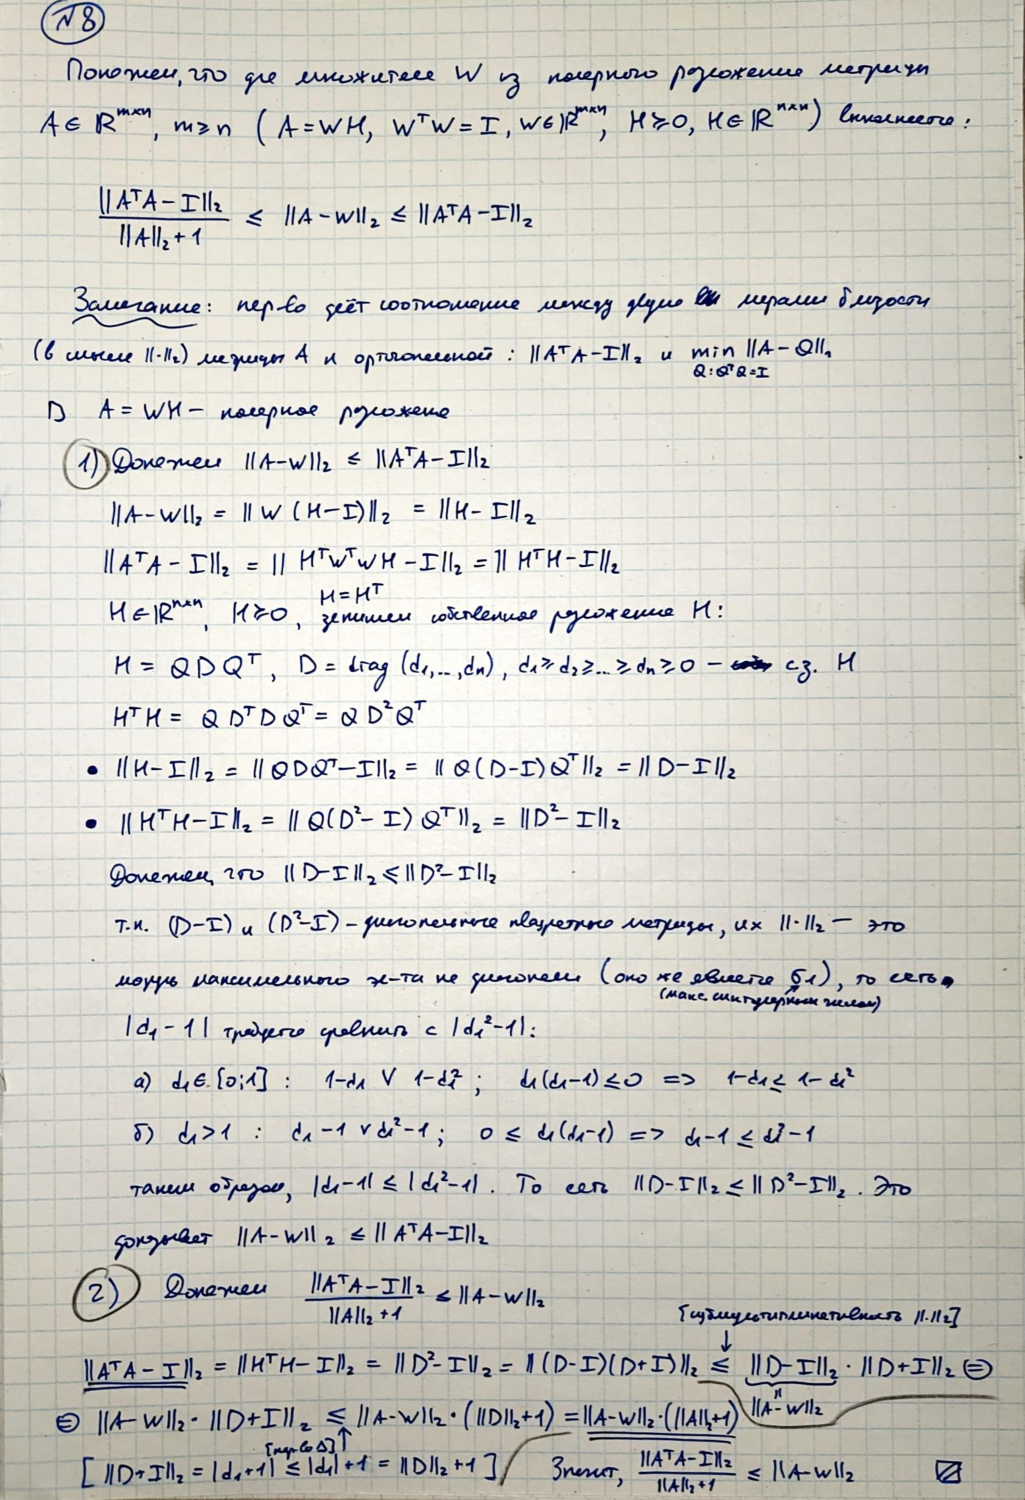
\includegraphics[width=0.95\linewidth]{handwritten/matcomp_hw1_8}
	\end{figure}
	
	\begin{figure}[h!]
		\centering
		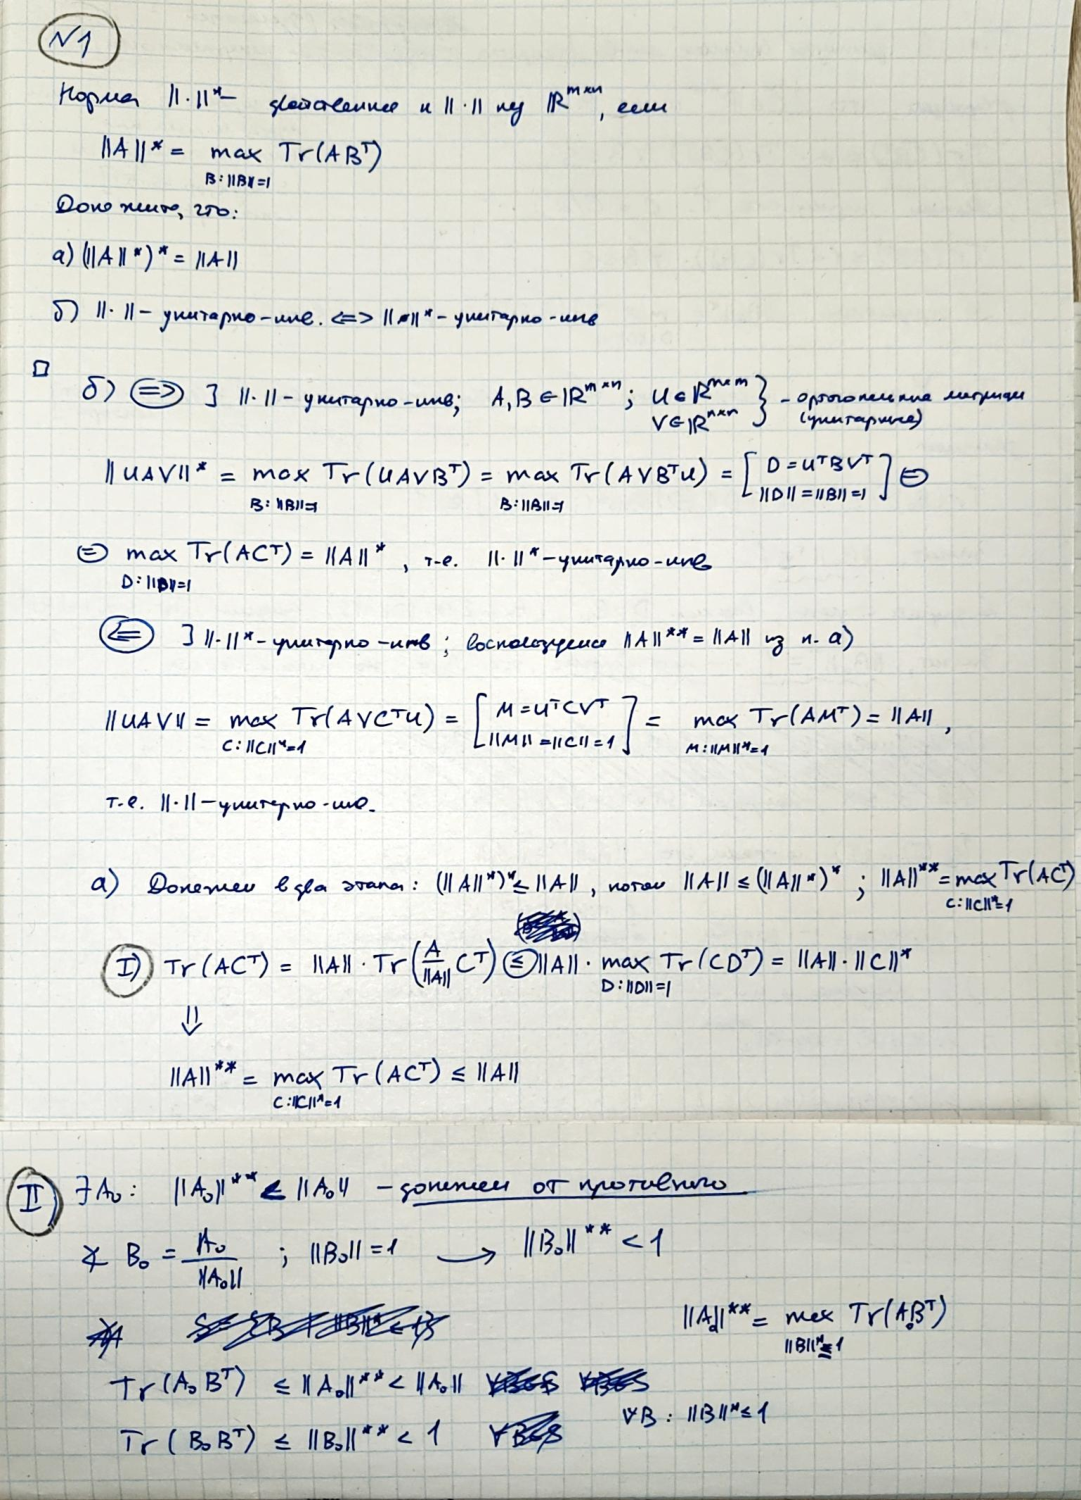
\includegraphics[width=0.95\linewidth]{handwritten/matcomp_hw1_bonus_1a}
	\end{figure}
	
	\begin{figure}[h!]
		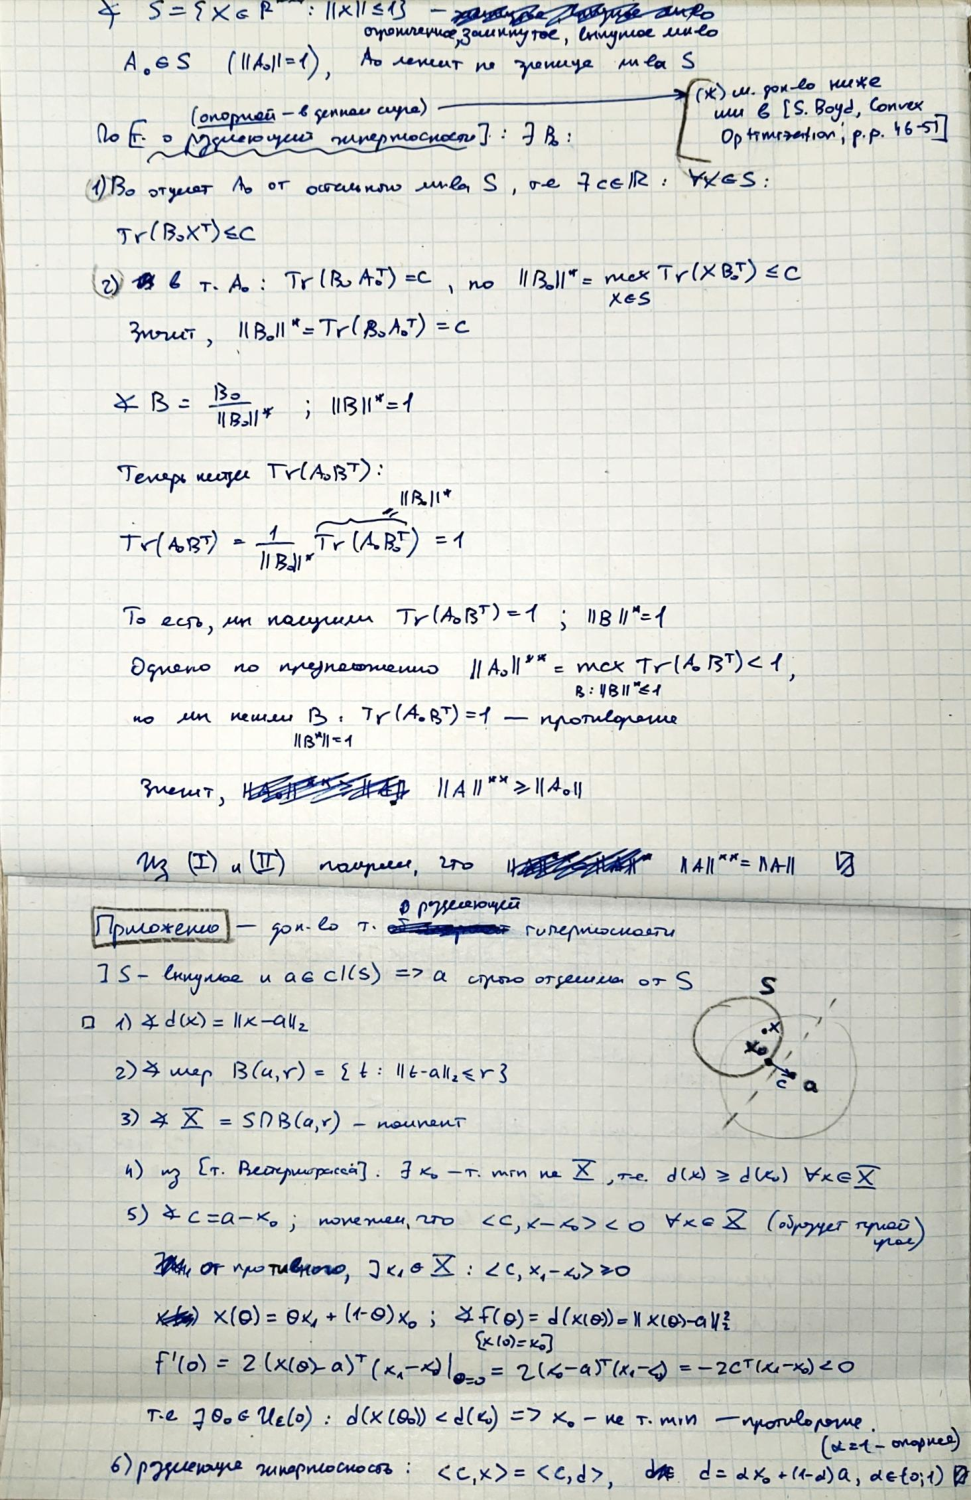
\includegraphics[width=0.95\linewidth]{handwritten/matcomp_hw1_bonus_1b}
	\end{figure}
	
	\begin{figure}[h!]
		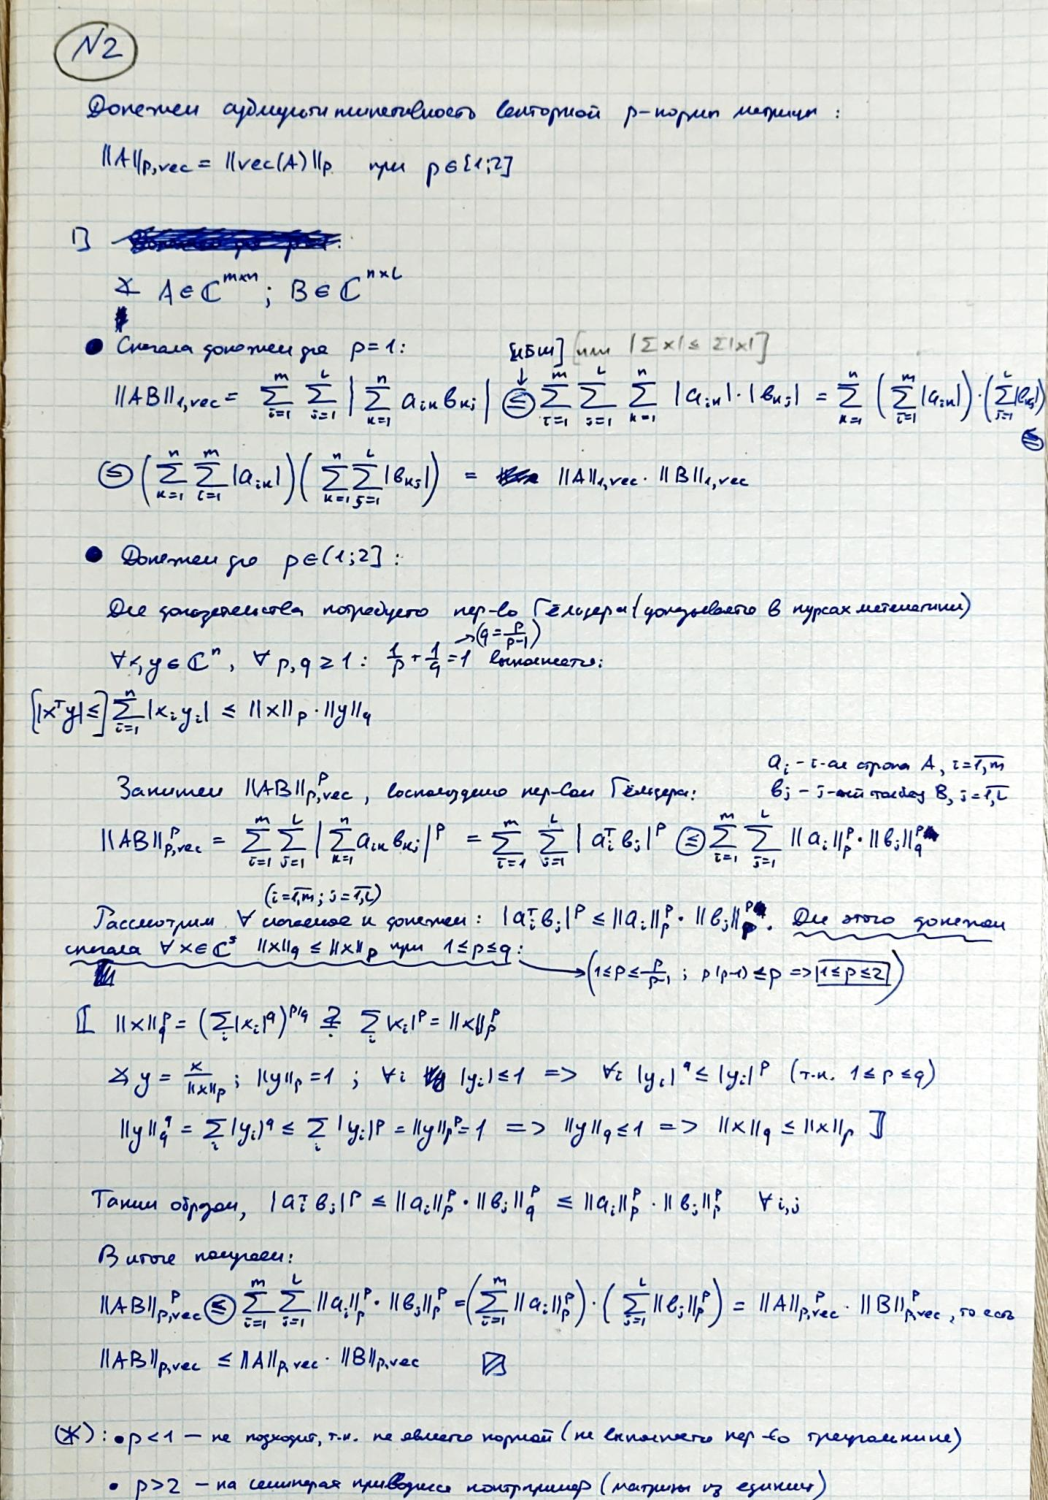
\includegraphics[width=0.95\linewidth]{handwritten/matcomp_hw1_bonus_2}
	\end{figure}
	
	\begin{figure}[h!]
		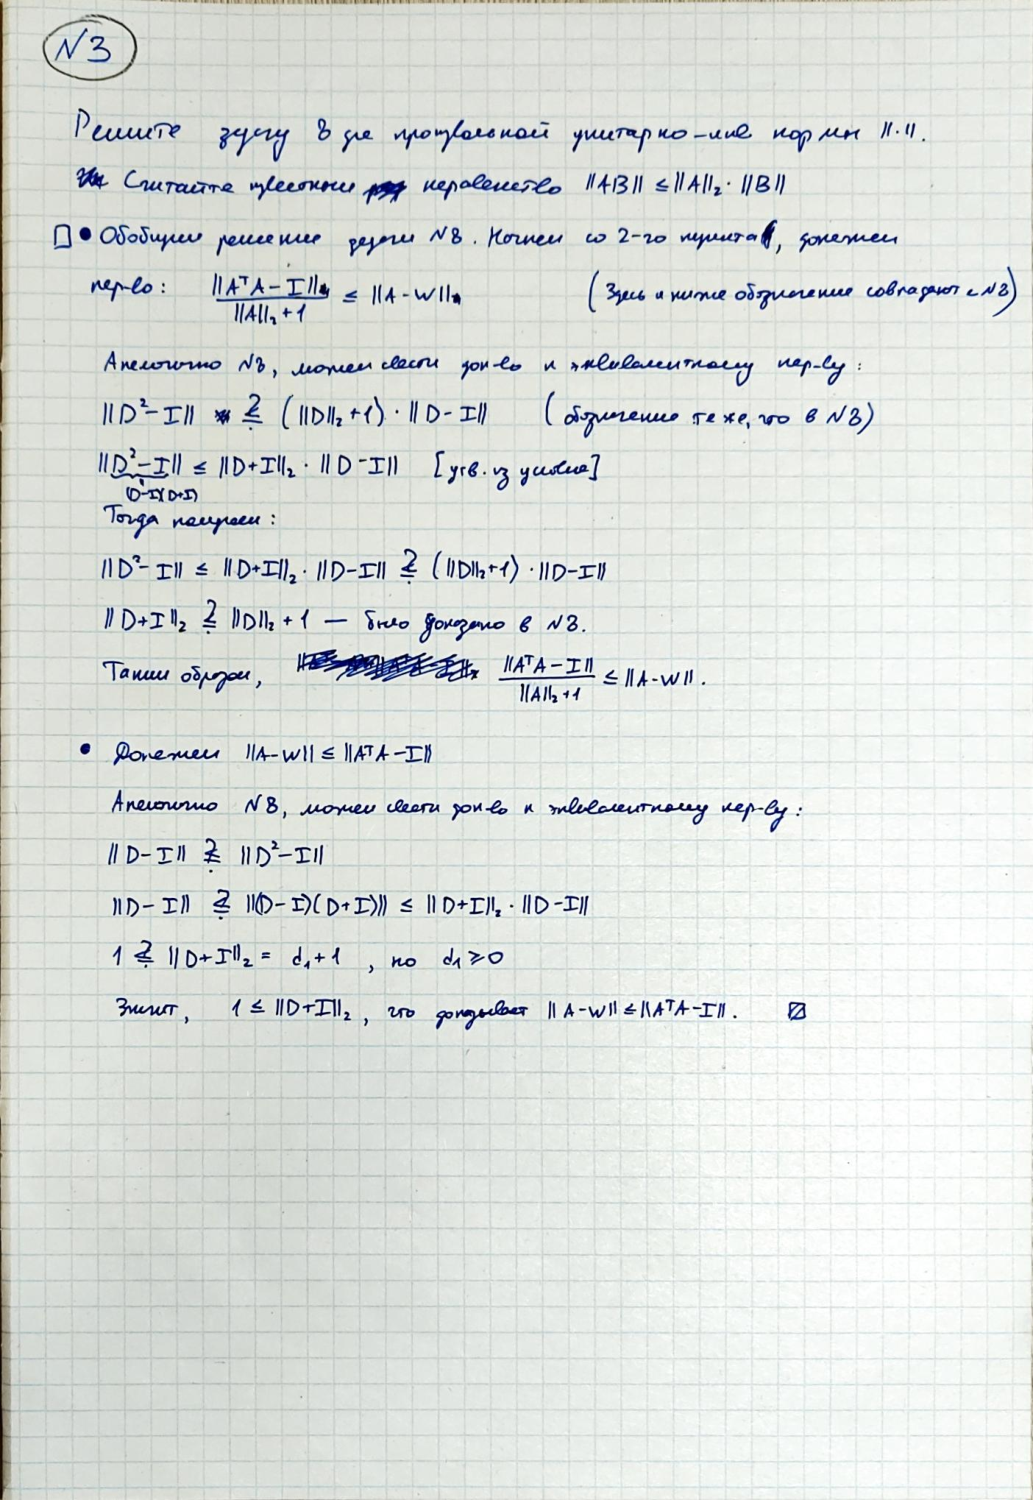
\includegraphics[width=0.95\linewidth]{handwritten/matcomp_hw1_bonus_3}
	\end{figure}
\end{document}
